\section{The final design}\label{sec:final-design}
The final design of the application will be discussed in the following section.
In \autoref{sec:sprint1-prototypes} an initial set of prototypes were defined to provide a vision for the design of the project, and the final design will be compared to these.
\begin{figure}[H]
    \centering
    \begin{subfigure}{0.45\textwidth}
        \centering
        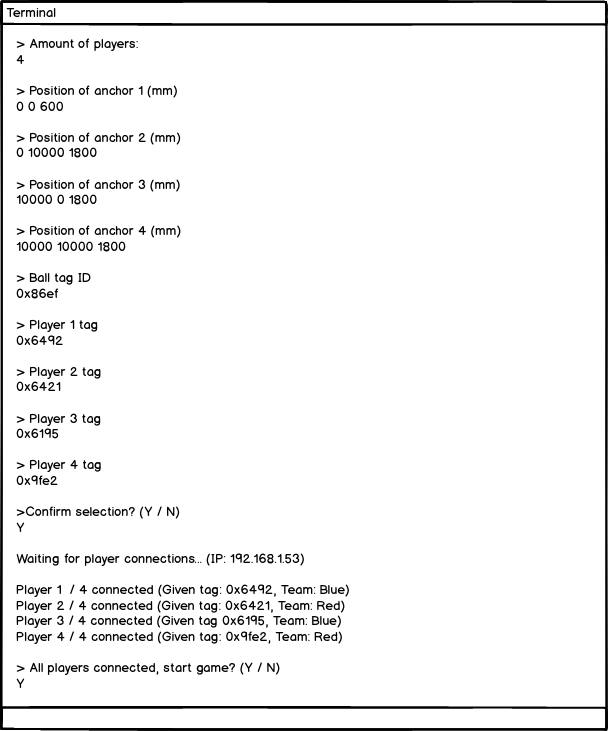
\includegraphics[width=0.8\linewidth]{prototypes/hostlobby.png}
        \caption{The prototype for the host to input data.}
        \label{fig:host-prototype}
    \end{subfigure}
    \begin{subfigure}{0.45\textwidth}
        \centering
        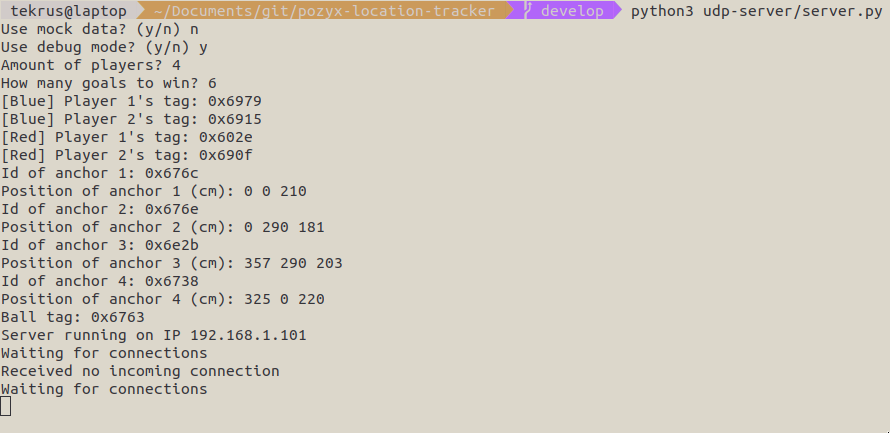
\includegraphics[width=1\linewidth]{sprint5/hostexample.png}
        \caption{The host interface for inputting data.}
        \label{fig:host-interface}
    \end{subfigure}
    \caption{The prototype and interface for the host.}
    \label{fig:comparing-host}
\end{figure}
\noindent
\autoref{fig:comparing-host} shows a comparison of the prototype for inputting data as well as its final design.
These do not differ substantially and are mainly focused on inputting text.
The main difference is that the implementation is more compact, such that the users can easily see their previous input.

\begin{figure}[H]
    \centering
    \begin{subfigure}{0.45\textwidth}
        \centering
        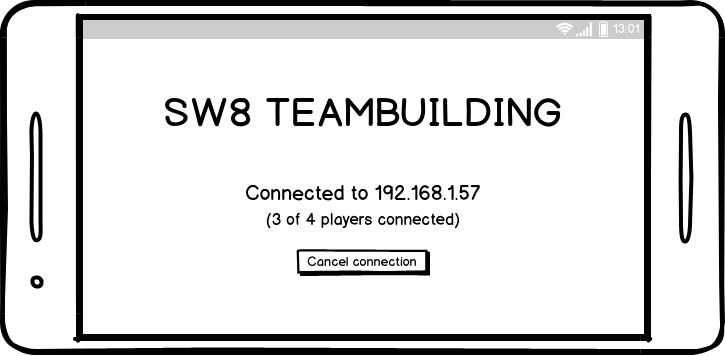
\includegraphics[width=0.8\linewidth]{prototypes/menuconnected.png}
        \caption{The prototype for players having connected.}
        \label{fig:connected-prototype}
    \end{subfigure}
    \begin{subfigure}{0.45\textwidth}
        \centering
        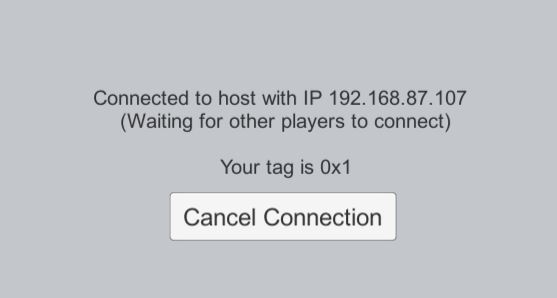
\includegraphics[width=0.8\linewidth]{sprint5/joinedgame.JPG}
        \caption{The implementation of players having connected.}
        \label{fig:connected-implementation}
    \end{subfigure}
    \caption{The prototype and implementation of the connected screen.}
    \label{fig:comparing-connection}
\end{figure}
\noindent
When players connect to a host they need to be made aware that it was successful.
\autoref{fig:comparing-connection} shows the prototype for this screen, as well as what it looks like in the final design.
They are mostly similar, but the final design adds text to make the player aware of which tag they should use.
The main difference is that the prototype shows how many players have connected to the game.
The game will be played exclusively as a local game, meaning the players could easily ask the host how many have connected so far, thus rendering the information on the screen rather useless since the player count will usually just be 2 or 4 players.
\autoref{fig:comparing-connection} aims to have a flat design, as defined in \autoref{sec:sprint1-prototypes}.

\begin{figure}[H]
    \centering
    \begin{subfigure}{0.45\textwidth}
        \centering
        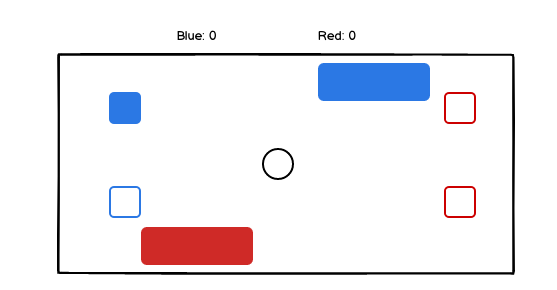
\includegraphics[width=0.8\linewidth]{prototypes/ingame.png}
        \caption{The prototype for playing the game.}
        \label{fig:ingame-prototype}
    \end{subfigure}
    \begin{subfigure}{0.45\textwidth}
        \centering
        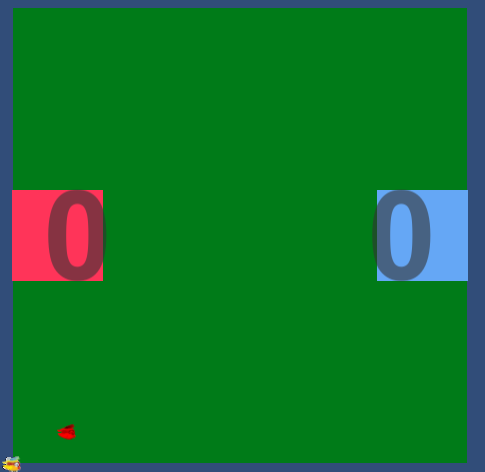
\includegraphics[width=0.8\linewidth]{figures/sprint-4-game.PNG}
        \caption{The final design of the game.}
        \label{fig:ingame-implementation}
    \end{subfigure}
    \caption{The prototype and implemented design of the in game scene.}
    \label{fig:comparing-ingame}
\end{figure}
\noindent
Finally, \autoref{fig:comparing-ingame} shows the prototype for playing the game as well as the final design implemented in Unity.
Section \ref{sec:sprint1-prototypes} introduced skeuomorphism, and defined that it was going to be used for the game design.
One way of realizing this was by making the field green, to represent grass.
Another way was to represent players as certain figures.
\autoref{fig:ingame-implementation} shows an example, being the birds in the corner.
Goals are red and blue, to show that each goal belongs to one team.
The big numbers represent number of goals.
The figure used for comparison has these overlapping with the goal zones.
This is not intended, and it has been changed such that the numbers are on the field close to the goals, but not overlapping.
If the players were to play on a field that was vertical, the goal zones would appear in the top and the bottom of the field, and the goal numbers would move along with them.
\autoref{fig:design-vertical} illustrates this.
\begin{figure}[H]
    \centering
    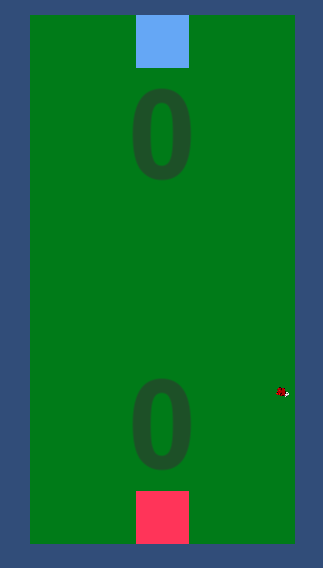
\includegraphics[width=0.2\linewidth]{sprint5/verticalgoals.png}
    \caption{Showing the design when the field is vertical.}
    \label{fig:design-vertical}
\end{figure}

\subsection{Concluding on the design}
The overall design achieves the vision of the prototypes.
The design also makes use of both flat and skeuomorphic design.
One issue with the current design if the game were to be played by users is that the only way to connect to a game is through manual input of the IP on which the game is being hosted.
This is not viable, and in case the game were to be deployed, it should be changed to feature a lobby system, rather than this manual input, to facilitate ease of use for the players of the game.
The lobby system would likely be implemented through a zero configuration management protocol, as discussed in \autoref{sec:accessonnetwork}.